\begin{figure}[p]
\centering
\begin{tikzpicture}[>=Latex,font=\small,
 box/.style={draw=blue!40!black,rounded corners=2pt,align=center,text width=5.55cm,minimum height=1.45cm,inner sep=8pt,fill=blue!3},
 result/.style={box,fill=green!6,draw=green!40!black},
 arr/.style={->,draw=blue!55!black,thick}]
\node[box,text width=12.5cm,fill=violet!5] (scope) at (3.5,0)
 {\textbf{Scope:} order $n\ge2$, tensor rank $>2$, over $\C$\\Original two-term equations; total multiplier--equation degree};
\node[box] (split) at (3.5,-2.2) {\textbf{Exhaustive cases}\\Some flattening rank $>2$, or every flattening rank $\le2$};
\node[box] (minor) at (0,-4.6) {\textbf{Case A: inherited minor lemma}\\A nonzero $3\times3$ minor\\gives an upper certificate of degree $3n$};
\node[box] (geom) at (7,-4.6) {\textbf{Case B: classical geometry}\\Secant-two flattening theorem\\and tangent-space description};
\node[result] (transfer) at (7,-7.0) {\textbf{Projection and balanced transfer}\\Map the target to $W_3$; pull back\\the explicit degree-9 certificate};
\node[result] (upper) at (3.5,-9.3) {\textbf{Upper bound in every case}\\$\delta_2(T)\le3n$};
\node[box] (lower) at (0,-7.0) {\textbf{Inherited lower functional}\\Annihilates $h_JF_J$ when\\$\deg(h_JF_J)<3n$, but $L(1)=1$};
\node[result,text width=8cm] (exact) at (3.5,-11.7) {\textbf{Exact theorem}\\$\delta_2(T)=3n$ for every $\rank(T)>2$};
\draw[arr] (scope)--(split);
\draw[arr] (split.west)-|(minor.north);
\draw[arr] (split.east)-|(geom.north);
\draw[arr] (geom)--(transfer);
\draw[arr] (minor.west)--++(-.45,0)|-(upper.west);
\draw[arr] (transfer.south)|-(upper.east);
\draw[arr] (upper)--(exact);
\draw[arr] (lower.south)--++(0,-.7)--++(-3.3,0)|-(exact.west);
\end{tikzpicture}
\caption{Proof outline of the exact theorem, with the original-parameter scope attached throughout. Blue boxes denote inherited or classical inputs; green boxes show the certificate transfer and resulting bounds. The two upper routes are conditional arguments combined by exhaustive cases; for $n=2$, only Case A occurs. The lower functional and either applicable upper route yield equality. Each box summarizes the indicated lemma or argument in \cref{app:math}; the companion expands its recorded premises.}
\label{fig:certificate-proof}
\end{figure}

\begin{figure}[p]
\centering
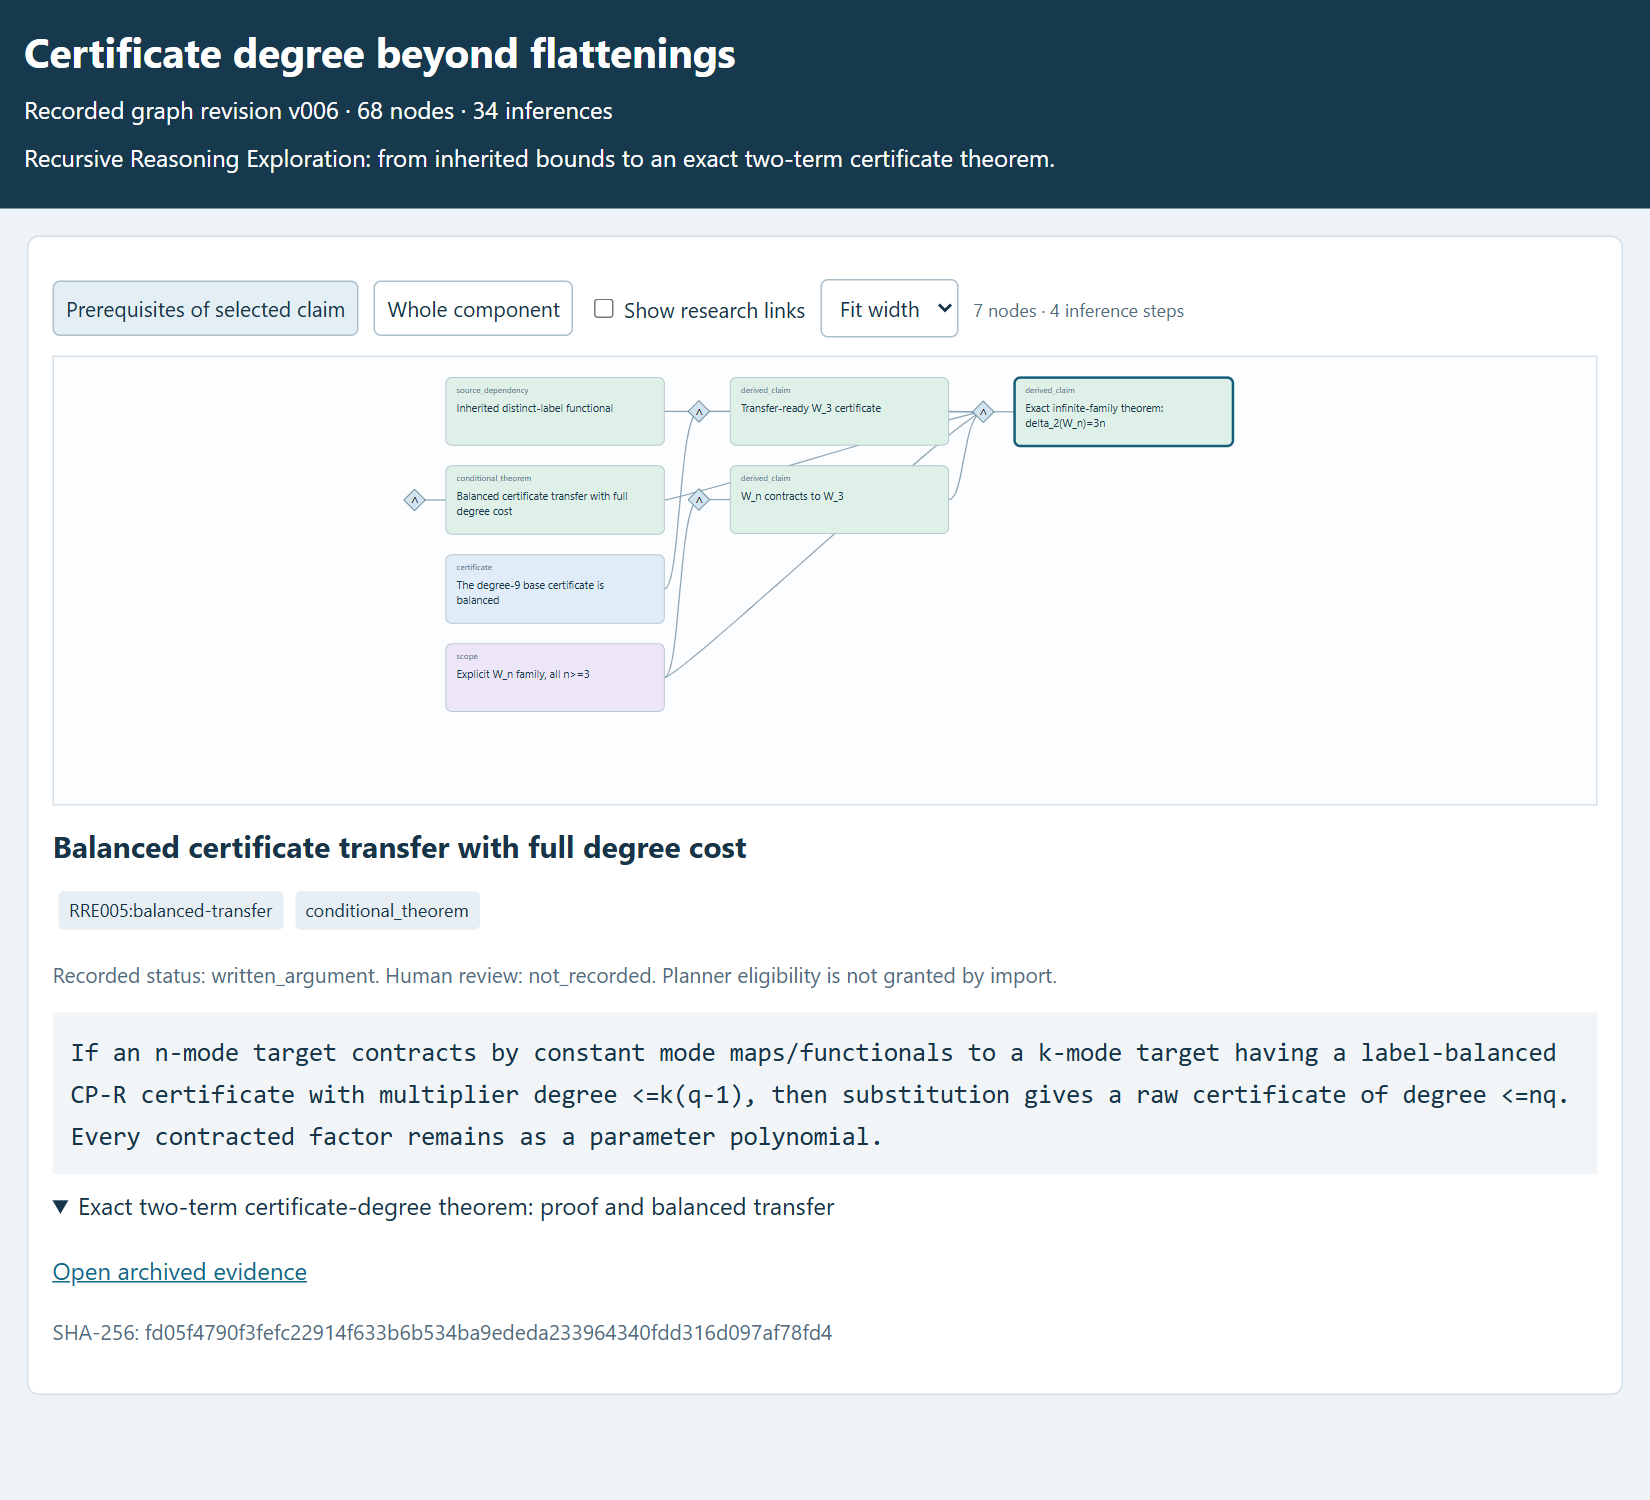
\includegraphics[width=\linewidth,height=.75\textheight,keepaspectratio]{figures/certificate_degree/inspector.png}
\caption{The implemented companion connects a selected graph record to its statement, scope, and hash-pinned evidence. The view focuses on the balanced transfer used to extend the boundary certificate. It is an interface excerpt; the versioned companion provides the full graph and prerequisite traces.}
\label{fig:certificate-inspector}
\end{figure}
